\chapter{Demo final}

\section{Introducción}

Hasta ahora hemos estado revisando algunos de los efectos gráficos más conocidos y comunes en el mundo de la \emph{demoscene}, analizándolos desde el punto de vista más analítico posible pero también intentando comprender su esencia y trasfondo.\\

Los efectos gráficos son el pilar, la base, que construye el mundo de la \emph{demoscene}, pero un solo efecto no hace una demo, pues una demo consiste en un conjunto de efectos gráficos compilados en un solo ejecutable, normalmente acompañados además de música que se reproduce de forma sincronizada.\\

Tras haber estudiado todos los efectos expuestos anteriormente, llega el momento de utilizar el conocimiento adquirido para intentar generar un obra, una \textbf{demo}, lo más interesante posible. Para ello, será necesario no sólo aplicar lo aprendido, si no también saber hacerlo de una forma que tenga una cierta coherencia en conjunto, de modo que resulte visualmente agradable. No hemos de olvidar que al fin y al cabo la \emph{demoscene} es tanto una práctica de ingeniería como de arte.\\

Si bien en este trabajo para nada se aspira a lograr una obra de arte, sí que se perseguirá un cierto sentido estético a lo largo de la composición, de forma que la compilación de todas las demos anteriores resulte lo más coherente y orgánica posible.\\

Como referencias a esta demo se pueden tomar todas aquellas que se han citado y mostrado previamente, pues esta demo pretende ser un humilde tributo y una humilde revisión de la cultura de la \emph{demoscene}, yendo a sus orígenes y efectos más clásicos y trayéndolos de vuelta a los computadores de hoy en día, ejecutando únicamente por CPU y en tiempo real.\\

\section{Planteamiento inicial}

Para desarrollar esta demo hay varias limitaciones o retos de base que nos debemos plantear. En primer lugar, la música juega un factor clave en las demos, y sin embargo hasta ahora no tenemos ningún mecanismo para generar sonido.\\

Además, la demo se ejecutará exclusivamente en la CPU del ordenador, lo cual si bien resulta muy interesante, dado que pone en valor las capacidades de cómputo de un ordenador, también resulta un factor limitante, pues la manipulación de millones de píxeles por segundo no es una tarea trivial, y aún menos si hay operaciones matemáticas complejas de por medio. Es por ello que deberemos aplicar todo lo aprendido para tratar de optimizar y estirar el rendimiento al máximo, y cuando esto no sea posible, buscar otras opciones o caminos que enmascaren las limitaciones técnicas de la máquina.\\

Por otro lado, los efectos gráficos que hemos mostrado hasta ahora son tan sólo muestras simplificadas de modo que resulten lo más explícitas y entendibles posible, pero ahora es el momento de buscar resultados más complejos o interesantes a partir de la base que ya ha sido planteada.\\

Por último, los efectos gráficos creados hasta el momento son bastante distintos o inconexos entre sí, por lo que será importante encontrar un modo orgánico de generar transiciones entre los mismos o combinarlos de una forma coherente.\\

A grandes rasgos, estas son las tareas necesarias para elaborar nuestra demo final:

\begin{itemize}
	\item Permitir la generación de sonido o música
	\item Aplicar o combinar todos y cada uno de los efectos gráficos explicados anteriormente
	\item Aplicar música a la demo coordinada con los efectos gráficos
\end{itemize}

\section{Generar sonido}

Antes de saltar a la implementación, conviene explicar muy brevemente como se representa el sonido de forma digital. Se asume, no obstante, que se conoce de forma básica el funcionamiento del sonido (física de ondas) y su representación matemática. Como ya sabemos, el sonido no es más que una vibración, una oscilación y por tanto, un movimiento ondulatorio. Si se requiere de un breve repaso sobre el funcionamiento de una onda, se puede encontrar en el planteamiento formal del efecto de deformaciones de imagen [\ref{sec:deformaciones}]\\

\begin{figure}[h]
	\centering
	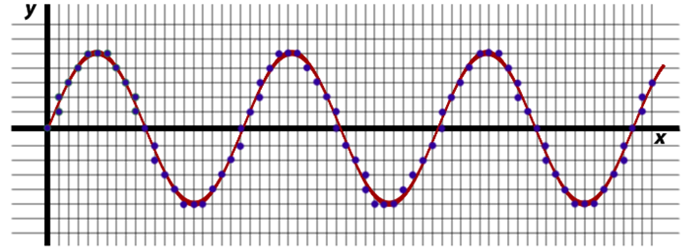
\includegraphics[width=13cm]{archivos/soundWave}
	\caption{Onda sinusoidal y su discretización}
	\label{fig:soundWave}
\end{figure}

Como podemos ver en la figura [\ref{fig:soundWave}], un sonido se puede representar como una onda (o una combinación de ondas). En el dominio analógico (en rojo), una onda es continua, sin embargo, en el dominio digital (en azul) solo se puede representar una cantidad discreta de valores de la onda, con la consiguiente pérdida de precisión. Es por ello, que para almacenar una onda en el dominio digital definimos una frecuencia de muestreo (equivalente a las líneas verticales de la imagen) y un formato o resolución de muestra (equivalente a las líneas horizontal en la imagen) de modo que cualquier valor intermedio, que no pueda ser representado, será aproximado al valor más cercano.\\

Habiendo dejado esto claro, pasamos a intentar generar sonido por computador. Siguiendo con la dinámica general de este trabajo, la generación de sonido debería ser, en la medida de lo razonable, gestionada por nosotros. La idea inicial es la de usar una librería de sonido para la música del mismo modo que usamos OpenGL para los gráficos, es decir, usar una librería que actúe simplemente como envoltorio y nos genere una capa de abstracción con respecto al sistema operativo, pero una vez hecho esto, generar el sonido desde cero.\\

Tras una breve investigación, las dos opciones más factibles parecían OpenAL\footnote{\url{https://www.openal.org}} y PortAudio\footnote{\url{http://www.portaudio.com}}. Si bien OpenAL es el equivalente directo de OpenGL pero para audio, PortAudio acabó siendo la librería elegida. OpenAL es una librería más estandarizada y potente, que permite generar sonido en 3D y tiene un modo de funcionamiento similar al de su casi homónimo OpenGL. Pero esta potencia viene al coste de una mayor complejidad de uso. PortAudio, en cambio, siendo una librería también de código abierto y multiplataforma, se centra en la simplicidad. Y por ello mismo se optó por ella, ya que parecía innecesario tener que aprender a manejar toda una librería potente y completa con el mero objetivo de usarla como una abstracción de cara al sistema operativo.\\

Una vez tenemos la librería elegida, llega el momento de empezar a implementar nuestro sistema capaz de generar sonido. Todo lo que PortAudio necesita para empezar a funcionar es inicializar la librería y crear un flujo (\emph{stream}) de sonido, al que se le pasa una función delegada controlada por el usuario.\\

\begin{lstlisting}[style=C-color, caption={Código necesario para inicializar PortAudio},label=cod:initialisePortAudio]
Pa_Initialize();
Pa_OpenDefaultStream(&stream, INPUT_CHANNELS, OUTPUT_CHANNELS, paFloat32, SAMPLE_RATE, FRAMES_PER_BUFFER, AudioCallback, 0);
Pa_StartStream(stream);
\end{lstlisting}

Para entender no obstante, cómo funciona PortAudio y los parámetros que nos pide, debemos entender cómo funciona el audio por computador. Como podemos ver en el código [\ref{cod:initialisePortAudio}], una vez inicializamos la librería, abrimos un flujo de sonido. Para hacer esto, no obstante, debemos pasar una serie de parámetros significativos. El primero de ellos, \emph{stream}, se trata simplemente de una estructura del tipo \emph{PaStream}. Esto es un tipo definido por los creadores de la librería y del que realmente no tendremos que preocuparnos, pues es gestionado internamente y no tendremos que realizar ningún tipo de operación con el mismo. La función principal de este tipo es la gestión de distintos canales de entrada y salida de sonido. A continuación debemos indicar los canales de entrada y de salida. Un canal de entrada se corresponde con una fuente de entrada de sonido. Aunque un canal no se corresponde necesariamente a un dispositivo, normalmente un canal de entrada se corresponde con un único dispositivo de grabación. Si en nuestra demo necesitásemos grabar audio, necesitaríamos entonces al menos un canal de entrada. Un canal de salida se corresponde normalmente, aunque no de forma necesaria, con un solo dispositivo de reproducción de audio, o en otras palabras, con un altavoz. Como en nuestra demo no necesitaremos grabar audio pero sí queremos reproducir audio estéreo, necesitaremos pues definir dos canales de salida.\\

Como nota, puntualizar que como se ha dicho anteriormente, un canal de entrada o salida no se corresponde necesariamente con un dispositivo físico. Esto es porque podemos por ejemplo definir dos canales de entrada que se correspondan con un único dispositivo de grabación, y sin embargo, dar a cada entrada de audio un tratamiento distinto. Por ejemplo, usar la entrada de un canal para generar eco y la del otro para generar distorsión, para posteriormente combinar los dos canales de entrada en un único canal de salida que tenga ambos efectos combinados. Del mismo modo, también es posible redirigir más de un canal al mismo dispositivo de reproducción. Por tanto, no existe una correspondencia directa entra canal y dispositivo, si bien es cierto que en muchos casos la suele haber.\\

Volviendo al código en [\ref{cod:initialisePortAudio}], una vez hemos definido que queremos dos canales de salida, llega el momento de definir el formato de muestra. Esto es, definir qué formato tendrá una única muestra de sonido. El valor de una muestra representa el valor de la amplitud del sonido en un instante dado. El sonido de los primeros ordenadores, el tan conocido como \emph{música de 8 bits}, tenía un formato de 8 bits interpretados como un entero por muestra. Esto quiere decir que la unidad mínima de sonido reproducible ocupaba 8 bits, y por tanto podía tener 256 valores distintos para la amplitud, que, para tratarse de sonido, podemos apreciar que es una resolución muy baja. De ahí que la música de 8 bits sonase robótica y poco orgánica, entre otras causas. De hecho, la música en 8 bits tan solo permitía 128 valores distintos, si tenemos en cuenta que en una onda que oscila en el origen, la mitad de los valores están por encima del cero y la otra mitad por debajo, por lo que de forma efectiva, contamos con 128 valores y su equivalente negativo. La música en 16 bits, que fue el siguiente paso, ya permitía definir más de 64000 valores distintos para la amplitud. Si escuchamos de hecho la diferencia entre la música de 16 bits y la música de 8 bits, se denota un cambio significativo. El formato que nosotros definimos en nuestra demo, no obstante, es el de un número en coma flotante de 32 bits. Nuestra amplitud máxima será 1 y nuestra amplitud mínima del sonido generado será -1. No obstante, como trataremos con números decimales, dispondremos de una gran resolución.\\

A continuación, una vez definido el formato de muestra (cuántos bits por muestra y cómo se deben interpretar -entero, coma fija, coma flotante...-) definimos el ratio de muestra, comúnmente denominado como la \emph{frecuencia de muestreo}, o en otras palabras, cuántas muestras queremos por segundo. Tal y como indica el teorema del muestro de Nyquist\footnote{\url{https://es.wikipedia.org/wiki/Teorema_de_muestreo_de_Nyquist-Shannon}}, para generar un sonido a una frecuencia determinada, necesitamos al menos el doble de muestras por segundo que la frecuencia que se pretende muestrear. De media, el ser humano es capaz de percibir frecuencias de entre 20 y 20000 Hercios, de modo que si queremos tener la habilidad de generar cualquier frecuencia audible, necesitaremos al menos 400000 muestras por segundo. En nuestra demo definimos una frecuencia de muestreo de 44100 muestras por segundo. El motivo de la elección de este número se debe a motivos históricos, ya que era la frecuencia de muestreo de los CD, ligeramente superior al espectro de sonido audible por cuestiones de formato y conveniencia\footnote{\url{https://es.wikipedia.org/wiki/Frecuencia_de_muestreo}}.\\

A continuación debemos definir la cantidad de muestras por \emph{buffer}. Como acabamos de explicar, para reproducir un sonido en cualquier frecuencia audible, es necesario contar con al menos 40000 muestras por segundo, y en nuestro caso definimos 44100 muestras de sonido por segundo. Pasar estas muestras una a una sería extremadamente poco eficiente, por no decir imposible. La tarjeta de sonido es la encargada de generar y reproducir audio, de modo que cada vez que reproducimos audio, la CPU debe comunicarse con la tarjeta de sonido. 40000 accesos por segundo a la tarjeta de sonido para enviar un solo dato es una locura, y muy lento. Es por ello que se define un \emph{buffer}. Cuando la CPU le pasa datos a la tarjeta de sonido, no lo hace de uno en uno, si no que manda la información en bloques de datos, reduciendo así la cantidad de comunicaciones con la tarjeta de sonido, que son operaciones bloqueantes. Con este parámetro, podemos definir el tamaño de los bloques de datos que se le pasan a la tarjeta de sonido. Bloques muy pequeños implican muchos accesos a la tarjeta de sonido, bloques muy grandes implican una gran cantidad de datos que transferir y una tasa de actualización muy baja (dado que nuestra función delegada se encarga de generar un bloque de datos por llamada, contando con la información en el momento de llamada, por lo que si esta información se actualiza a mitad de la generación de un bloque, la actualización no se verá reflejada hasta la siguiente llamada a nuestra función). Por tanto, conviene elegir un tamaño de \emph{buffer} que resulte razonable, ni demasiado pequeño, ni excesivo. En nuestra demo definimos un tamaño de 256 muestras por \emph{buffer}, lo que se traduce en unos 170 accesos a la tarjeta de sonido por segundo, y unas 170 llamadas a nuestra función delegada por segundo. Del mismo modo, el tamaño de cada \emph{buffer} será de 2KB (4 bytes -32 bits- por muestra, dos canales, 256 muestras por  canal por \emph{buffer}), un tamaño que no resulta trivial pero que es muy pequeño.\\

Tras ello, los siguientes dos parámetros que hemos de pasar son una función delegada a la que PortAudio llamará de forma interna para generar sonido y, de forma opcional, una estructura definida por el usuario. En nuestro caso, realizaremos todas las operaciones necesarias desde la función delegada, y tenemos todos los datos que necesitamos en nuestra clase. Podremos acceder a estos datos desde nuestra función delegada, ya que es un miembro estático de nuestra clase para reproducir audio. Por tanto, pasaremos un 0 (también sería posible y equivalente en este caso pasar un \emph{nullptr}) para indicar que no haremos uso de ninguna estructura de datos definida por el usuario.\\

Llega ahora el momento de echar un vistazo a la función delegada que puede ser definida por el usuario:\\

\begin{lstlisting}[style=C-color, caption={Función delegada que pasamos a PortAudio},label=cod:audioCallback, escapechar=|]
int Imp_Audio::AudioCallback(const void *inputBuffer, void *outputBuffer,
                             unsigned long framesPerBuffer,
                             const PaStreamCallbackTimeInfo *timeInfo,
                             PaStreamCallbackFlags statusFlags,
                             void *userData)
{
    float *out = (float *)outputBuffer;
    static long int currentCount = 0;

    for (unsigned long i = 0; i < framesPerBuffer; i++)
    {
        currentCount++;

        Imp_Audio::UpdateNotes(currentCount);

        *out++ = Imp_Audio::GetLeftValue();  /* left */ | \label{line:left}|
        *out++ = Imp_Audio::GetRightValue(); /* rigth */| \label{line:right}|
    }
    return 0;
}
\end{lstlisting}

Aunque la cantidad de parámetros que recibe la función delegada puede abrumar a primera vista, la realidad es que apenas usamos unos pocos, como podemos ver en el código [\ref{cod:audioCallback}].\\

No usamos el \emph{inputBuffer}, dado que no hemos definido ningún canal de entrada, del mismo modo que tampoco usamos las variables \emph{timeInfo}, \emph{statusFlags} o \emph{userData}, las dos primeras porque son variables que nos aportan información extra pero que no nos resultan especialmente relevantes y la última porque es el argumento que se corresponde con la estructura de datos definida por el usuario que en nuestro caso hemos decidido no definir. Por tanto, sólo estamos interesados en dos variables, el \emph{outputBuffer}, que se corresponde con el \emph{buffer} para la salida de datos, es decir, es el \emph{buffer} cuyos datos son pasados a la tarjeta de sonido para ser reproducidos por el ordenador y por otro lado, la variable \emph{framesPerBuffer}, que recordemos que habíamos definido previamente con el valor 256 y que nos indica por cada llamada a la función, cuántas muestras por canal debemos incluir en el \emph{buffer}. Si nos fijamos en las líneas [\ref{line:left}] y [\ref{line:right}], veremos que en estas líneas asignamos un valor a la posición actual del \emph{buffer} y a continuación la incrementamos. Como podemos recordar, hemos definido dos canales de salida de audio, dado que queremos audio estéreo. Esto implica, por tanto, que nuestro \emph{buffer} deberá ser rellenado con muestras para ambos canales. Estas muestras se leen de forma intercalada, de modo que si visualizamos nuestro \emph{buffer} como un \emph{array}, su primer valor se corresponderá con la primera muestra del canal izquierdo, su segundo valor con la primera muestra del canal derecho, su tercer valor con la segunda muestra del canal izquierdo, y así sucesivamente... Esto nos permite, de forma bastante sencilla, asignar valores a nuestros canales de salida de audio.\\

Antes de continuar ahondando en el funcionamiento del sistema de sonido, vale la pena explicar su funcionamiento de forma genérica, a partir de lo previamente construido.\\

En nuestro sistema, tenemos un vector estático de notas. Podemos ver la estructura de una nota en la figura [\ref{fig:note}]. Por cada muestra que añadimos al \emph{buffer} de salida, actualizamos los valores de todas las notas que se están reproduciendo actualmente, basándonos en la variable entera \emph{currentCount}, que se actualiza por iteración. De esta modo, usamos \emph{currentCount} para actualizar el valor de nuestras notas de forma muy similar a como usamos el valor de \emph{deltaTime} para actualizar nuestras demos. De hecho, ambas variables tienen una relación directa con el tiempo, ya que \emph{deltaTime} representa el tiempo transcurrido desde el fotograma anterior mientras que \emph{currentCount} representa el número de muestra que se está actualizando, y como sabemos, actualizamos 44100 muestras por segundo, por lo que cada 44100 actualizaciones de este valor, habrá transcurrido un segundo.\\

Una vez actualizamos el valor de nuestras notas, llega el momento de asignarlas a la salida. Para ello, llamamos a dos funciones que respectivamente nos devolverán el valor para la salida de audio izquierda y el valor para la salida de audio derecha, basándose en la posición de las notas que se están reproduciendo actualmente.\\ 

%@startuml
%
%class Note << (S,#FF7700) Struct >>
%{
%  +float (*generateWave)(frequency, count)
%  +Envelope envelope
%  +float frequency
%  +float volume
%  +float position
%  +float lifetime
%  +float currentEnvelopeValue
%  +float resultingSound
%}
%
%class Envelope << (S,#FF7700) Struct >>
%{
%  +float attack
%  +float decay
%  +float sustain
%  +float release
%  +float peakAmplitude
%  +float sustainAmplitude
%  
%}
%
%hide empty members
%
%@enduml

\begin{figure}[h]
	\centering
	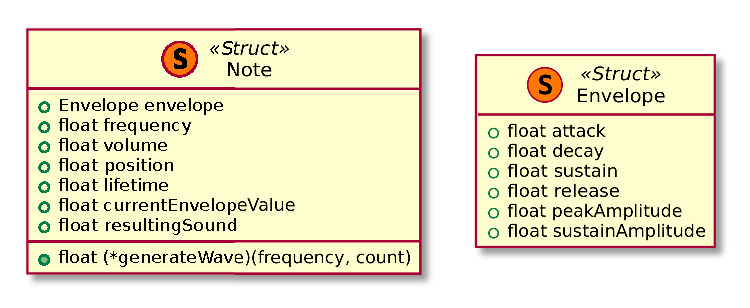
\includegraphics[width=13cm]{archivos/note}
	\caption{Estructura de una nota y su envolvente}
	\label{fig:note}
\end{figure}

Una vez que entendemos de forma simplificada como funciona nuestro sistema, llega el momento de definir qué es una nota y cómo se utiliza. Podemos ver su estructura en la figura [\ref{fig:note}].\\

Una nota musical se define principalmente por los siguientes parámetros: su forma de onda, su frecuencia, su volumen y su envolvente. La forma de onda en nuestro caso es generada por una función delegada, que a partir de la frecuencia deseada y el número de muestra, genera el valor correspondiente. De este modo, podemos asignar distintas formas de onda a distintas notas con gran facilidad, simplemente cambiando la función delegada de la misma. La frecuencia se corresponde con la frecuencia de la onda y el volumen con la amplitud, valor que oscilará entre 0 y 1. Por último, ya solo queda definir la envolvente, lo cual es algo más complejo.\\

La envolvente de una nota, o de un sonido en general, es algo así como "el ciclo de vida" de un sonido. Podemos ver la forma o estructura habitual de una envolvente en la figura [\ref{fig:ADSR}]. A este tipo de envolvente se la denomina comúnmente envolvente \emph{ADSR}, siendo estas siglas la denominación de las fases de la envolvente, en español, ataque, decaimiento, sostenimiento y relajación.\\

\begin{figure}[h]
	\centering
	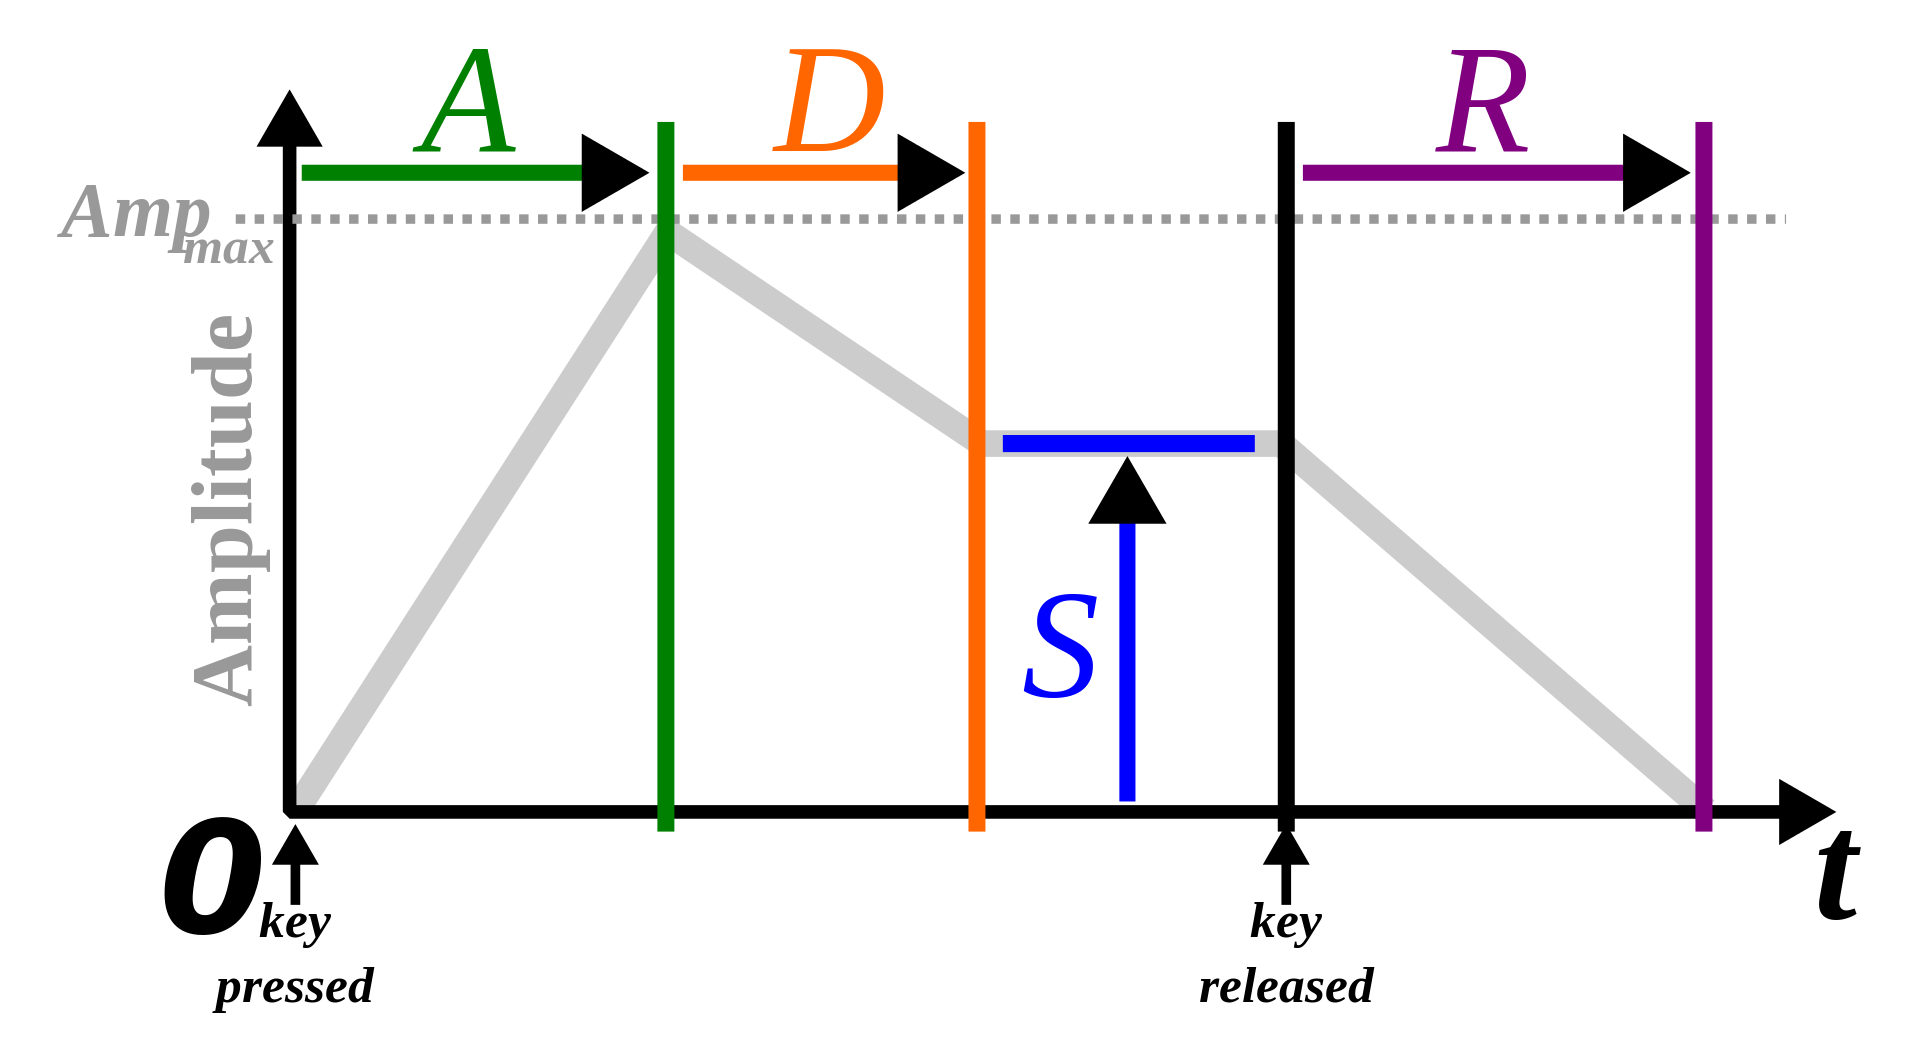
\includegraphics[width=10cm]{archivos/ADSR}
	\caption{Envolvente de un sonido - Fuente: \href{https://en.wikipedia.org/wiki/Envelope_(music)\#/media/File:ADSR_parameter.svg}{Wikipedia}, por \href{https://commons.wikimedia.org/wiki/User:Abdull}{Abdull}}
	\label{fig:ADSR}
\end{figure}

Vamos a clarificar qué es una envolvente con un ejemplo práctico: tocar una nota en un piano real. Cuando tocamos una nota en un piano, hay un momento en el que se pasa del silencio a emitir un sonido. Esta es la fase de ataque, que se produce en el instante en que el martillo golpea las cuerdas. Tras esto, la amplitud (volumen) de la nota decae levemente, siendo esta la fase de decaimiento, pero, si mantenemos la nota pulsada, sigue sonando a una amplitud inferior, siendo esta la fase de sostenimiento. Ya por último, una vez dejamos de presionar la tecla, o si pasa el tiempo suficiente, el sonido empieza a decaer hasta que se desvanece, entrando por tanto en la fase de relajación. Prácticamente todos los instrumentos tienen estas fases, en mayor o menor medida. La envolvente de un sonido, por tanto, define la evolución del volumen del sonido a lo largo del tiempo, y define de forma drástica la forma en la que suena un instrumento. Por ejemplo, si pulsamos una tecla en un piano lentamente no sonará igual que si la pulsamos de golpe, porque tendrá una fase de ataque distinta, siendo la segunda mucho más breve. Además de definir estas cuatro fases, definimos dos variables más, la amplitud máxima y la amplitud de sostenimiento. La primera define el volumen que la nota alcanza tras la fase de ataque. La segunda define el volumen de la nota una vez que este decae y se sostiene, en la fase de sostenimiento.\\

Por tanto, pues, cada vez que actualicemos el valor de nuestra nota, también deberemos actualizar el valor de la envolvente en el ciclo de vida actual de la nota. Para ello, simplemente debemos crear una función que sea capaz de interpolar entre estos estados. Es decir, dado un tiempo de ataque, debe interpolar entre el reposo (0) y la amplitud máxima, una vez que se alcanza esta amplitud y acaba la fase de ataque, el volumen de la nota decae en la fase de decaimiento tanto tiempo como se especifique hasta estabilizarse en la amplitud de sostenimiento, que se mantendrá constante durante toda esta fase. Tras ello, entraremos en la última fase y en el final del ciclo de la vida de la nota, donde pasamos de la amplitud de sostenimiento al reposo de nuevo, el silencio. Es en este momento cuando termina el ciclo de vida de la nota.\\

Por tanto, en la estructura de la nota, que podemos ver en la figura [\ref{fig:note}], las primeras cuatro variables contienen información constante sobre la nota que se está reproduciendo, mientras que las tres últimas contienen estado: el tiempo de vida de la nota (cuando el tiempo de vida de la nota es igual a la duración de la envolvente, se considera que la nota ha terminado y por tanto se elimina de nuestro vector de notas), el valor de la envolvente para el tiempo de vida actual, que dependerá de la fase de la envolvente en que nos encontremos y modificará el volumen de la nota y el sonido resultante, que se corresponde con el valor de retorno del método delegado que la nota contiene.\\

La única variable de la que aún no hemos hablado es en realidad una bastante interesante, la variable \emph{position}. El valor de esta variable oscila entre 0 y 1, 0 representando el canal izquierdo y e1 1 representando el canal derecho. El valor por defecto de esta variable es \(0.5\), que se corresponde al centro, o en otras palabras, nuestra nota sonando con la misma intensidad por el altavoz izquierdo y el derecho. Si asignamos a esta variable el valor 0, el sonido de nuestra nota se reproducirá solo por el canal izquierdo pero no por el derecho, y lo mismo se aplica a la inversa si aplicamos un valor de 1. Cualquier valor intermedio emitirá sonidos por ambos canales, tendiendo aquellos canales por debajo de \(0.5\) a la izquierda y aquellos por encima de \(0.5\) a la derecha.\\

Ahora que ya hemos explicado cómo funcionan las notas en nuestro sistema, podemos ver por fin el código para actualizarlas y reproducirlas por el canal izquierdo o derecho, como hacemos en el código [\ref{cod:audioCallback}].\\

\begin{lstlisting}[style=C-color, caption={Actualización y obtención del valor de las notas},label=cod:updateNotes, escapechar=|]
void Imp_Audio::UpdateNotes(long int currentCount)
{
    for (auto &note : notes)
    {
        note.resultingSound = note.generateWave(note.frequency, currentCount) * note.currentEnvelopeValue * note.volume;
    }
}

float Imp_Audio::GetLeftValue()
{
    float sum = 0.f;

    for (auto &note : notes)
    {
        float leftAmplitude = 1.f;
        if (note.position > 0.5f)
        {
            leftAmplitude -= (note.position - 0.5f) * 2.f;
        }

        sum += note.resultingSound * leftAmplitude;
    }

    return sum;
}
\end{lstlisting}

En el código [\ref{cod:updateNotes}] se aporta el método para actualizar notas y el método para obtener el valor de muestra para el canal izquierdo. Se omite el del canal derecho ya que es prácticamente equivalente en funcionalidad al del izquierdo.\\

Para actualizar el valor de una nota, lo que hacemos es multiplicar el resultado que nos devuelve nuestro método delegado (en función de la frecuencia y el tiempo actual) por el valor actual de la envolvente de la nota y el volumen general de la nota. Las envolventes no se actualizan en este bucle, si no que son actualizadas en la función \emph{Update} de la propia clase, en lugar de actualizarse dentro de la función delegada que es gestionada por PortAudio. Esta decisión se ha tomado de modo que sea más fácil gestionar la actualización de la envolvente, que depende directamente del tiempo, por lo que es más fácil de actualizar con un intervalo de tiempo (\emph{deltaTime}) que no con un número de muestra (\emph{currentCount}) y también para aliviar la cantidad de cálculos, pues en lugar de tener que actualizar la envolvente por muestra (44100 veces por segundo) la actualizamos por fotograma (unas 60 veces por segundo). Esta decisión tiene sus ventajas e inconvenientes, pues por un lado implica no tener que estar constantemente actualizando la envolvente pero por otro, también facilita que se puedan producir pequeños cortes o cambios bruscos en la intensidad del sonido. En general, y bajo opinión personal, pienso que actualizando la envolvente una vez por fotograma el resultado es suficientemente satisfactorio, pero si se quisiera actualizar por muestra, sería tan sencillo como invocar a la función de actualizar envolvente en el bucle del código [\ref{cod:audioCallback}], pasándole por valor \(1 \div 44100\), es decir, la cantidad de tiempo que transcurre de una muestra hasta la siguiente.\\

A continuación, la función \emph{GetLeftValue} calcula el valor para el canal izquierdo por nota y lo suma. Si el valor de la variable \emph{position} de la nota se halla entre 0 y \(0.5\), entonces el factor  de amplitud en el canal izquierdo para esa nota será de 1, pero el factor para esa nota en el canal derecho será menor que 1. Del mismo modo, si la posición de la nota es superior a \(0.5\), entonces el factor de amplitud en el canal izquierdo será menor, o en otras palabras, la nota sonará con menor intensidad por el canal izquierdo. Por tanto, situada en el centro (\(0.5\)), una nota sonará con su amplitud natural tanto por el canal izquierdo como por el derecho, mientras que si no se sitúa en el centro, su amplitud será menor en un canal o en otro. Una versión refinada de esta implementación sería una el que que el módulo del sonido total de la nota siempre fuera 1, por lo que en el centro, el factor para el canal izquierdo y derecho sería \(\sqrt{\frac{1}{1 + 1}} = \sqrt{\frac{1}{2}} \approx 0.707\). No obstante, para evitar complejidad añadida y una mayor carga computacional, se ha optado por la solución que se muestra en código, más sencilla y con un resultado práctico similar.\\

Como podemos ver en la función \emph{GetLeftValue} en el código [\ref{cod:updateNotes}], el valor de cada nota se suma acumulativamente y se devuelve como el valor total para el canal. Recordemos que este valor se corresponde al de la amplitud general de la salida de sonido para el canal, por lo que debe estar comprendido entre -1 y 1. De lo contrario, si sobrepasamos este límite, se producirán artefactos de sonido extraños y desagrables, que en el peor de los casos podrían llegar incluso a dañar nuestros altavoces (aunque en nuestro caso no corremos ese riesgo, dado que PortAudio se encargará de filtrar todos aquellos valores que se salgan de rango). No obstante, queda en manos de quien añada sonidos asegurarse de que la suma de los sonidos no sobrepase el umbral máximo. Por ejemplo, si hacemos sonar dos instrumentos a la vez, deberíamos hacer que cada uno sonase a la mitad de su amplitud, de modo que sumados, como máximo, sumasen la amplitud máxima. De este modo, dejamos al usuario la decisión de la masterización del sonido, que si bien implica una responsabilidad (de lo contrario se producirán artefactos de sonido desagradables) también otorga una mayor flexibilidad.\\

Así pues, recapitulando, hemos creado un sistema que nos permite gestionar y reproducir notas de sonido complejas, con una envolvente asociada y en estéreo. No obstante, y antes de continuar a la siguiente sección, aun nos queda algo fundamental por definir, ¡una forma de generar ondas de sonido!\\

\begin{figure}[h]
	\centering
	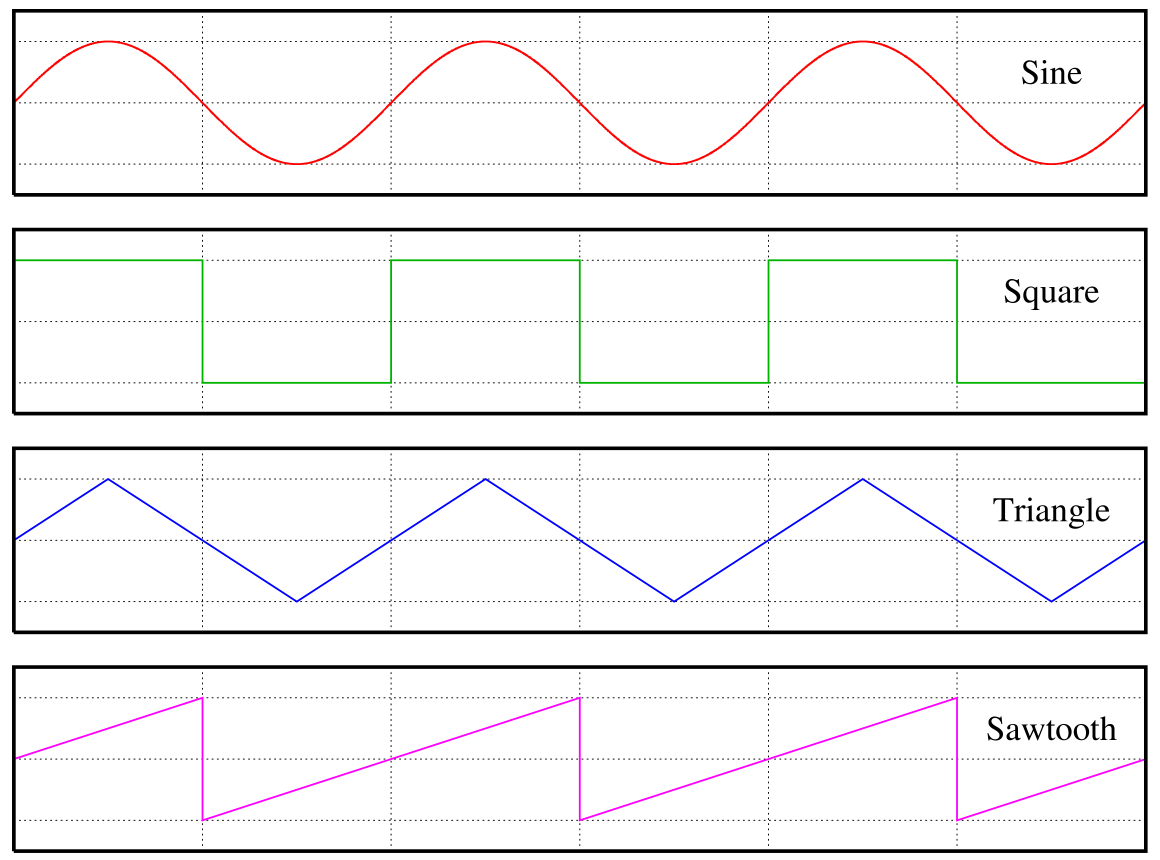
\includegraphics[width=10cm]{archivos/waves}
	\caption{Distintas formas de onda - Fuente: \href{https://upload.wikimedia.org/wikipedia/commons/6/6f/Waveforms.png}{Wikipedia}, por \href{https://commons.wikimedia.org/wiki/User:Omegatron}{Omegatron}}
	\label{fig:waves}
\end{figure}

Históricamente, encontramos cuatro tipos distintos de ondas generadas por ordenador, que podemos ver en la figura [\ref{fig:waves}]. La onda cuadrada y la de diente de sierra son ondas que suenan muy robóticas o metálicas, por tanto muy lejanas al sonido natural. Sin embargo, son muy fáciles de calcular, ya que tienen un muy bajo coste computacional, por lo que los primeros ordenadores y videoconsolas que podían generar sonido, tenían capacidad para generar sólo este tipo de ondas. Al fin y al cabo, para generar un sonido se requiere una gran cantidad de muestras por segundo, por lo que en un ordenador de poca potencia, el cálculo para hallar el valor de una muestra debe ser lo más rápido posible, o de lo contrario, ralentizará la ejecución del programa. Es por ello, por tanto, que se generaban ondas cuadradas (que oscilan entre dos únicos valores, \emph{+amplitud} y \emph{-amplitud}) y las ondas de diente de sierra, cuyo valor de la amplitud se incrementa a lo largo de la longitud de la onda para decaer a 0 al final de cada iteración.\\

Las ondas triangulares son ondas que, siendo mucho más sencillas de calcular que una onda sinusoidal, resultan mucho más orgánicas que las dos anteriores, pues consiste en una interpolación continua entre la amplitud máxima y la máxima negativa. Tiene una carga de cómputo algo más elevada que la de las ondas cuadrada y de diente de sierra pero, sin embargo, ofrece un resultado sonoro bastante más orgánico a un coste relativamente bajo.\\

Por último tenemos las ondas sinusoidales. En la naturaleza, o en el mundo real, el sonido se propaga de manera natural con esta forma de onda. Sin embargo, como bien sabemos, el cálculo del seno es una operación matemática para nada trivial, por lo que este tipo de onda tardaría un tiempo en llegar a los ordenadores. Siempre se podría usar tablas precalculadas en lugar de la operación matemática, pero recordemos que el uso de tablas precalculadas también introduce un cierto factor de complejidad y un error añadido, por su limitación en precisión. Nuevamente, la elección de un técnica u otra depende de la consideración personal.\\

\begin{lstlisting}[style=C-color, caption={Cálculo de una onda sinusoidal con una frecuencia determinada},label=cod:sineWave, escapechar=|]
float Sounds::GetSineWaveValue(float frequency, long int currentCount)
{
    int steps = SAMPLE_RATE / frequency;

    float percentage = currentCount % steps / float(steps);

    return sin(2 * Fast::PI * percentage);
}
\end{lstlisting}

En el código [\ref{cod:sineWave}] vemos la implementación de la función para generar ondas sinusoidales. Como podemos ver, cumple la signatura del método delegado de una nota [\ref{fig:note}], de modo que podemos hacer fácilmente que una nota reproduzca sonido con forma de onda sinusoidal.\\

El sonido que generamos depende de la frecuencia, por lo que lo primero que hacemos es calcular, para la frecuencia dada, la cantidad de muestras necesarias para generar un único ciclo o iteración de la onda. Este valor se corresponde con la frecuencia de muestreo dividida por la frecuencia deseada. Por ejemplo, si tenemos una frecuencia de muestreo de 2000 muestras por segundo y queremos emitir un sonido a 200 Hercios, por tanto, 200 oscilaciones por segundo, entonces se deberá producir una oscilación a cada \(\frac{2000}{200} = 10\) muestras.\\

Una vez hemos hallado la cantidad de muestras por oscilación, hallamos el punto o porcentaje en el que nos encontramos dentro de la oscilación. Para hacer esto, hallamos el módulo del número de muestra actual en función de la cantidad de muestras por oscilación y lo dividimos por la cantidad de muestras por oscilación. Por ejemplo, si estamos en la muestra 25 y tenemos 10 muestras por oscilación, entonces hallamos el módulo \(25\mod 10 = 5\) y lo dividimos entre la cantidad de muestras por oscilación \(\frac{5}{10} = 0.5\), hallando que nos encontramos a la mitad de la oscilación.\\

Una oscilación completa equivale a una circunferencia completa, es decir, \(2\pi\), por lo que sabiendo el punto de la oscilación en que nos encontramos, sólo tenemos que multiplicar por \(2\pi\) y calcular el seno del valor obtenido para hallar la amplitud de nuestra onda a una frecuencia determinada en un instante de tiempo dado.\\

Podríamos pensar que ya hemos acabado con la generación de sonido, pero aún nos queda ser capaces de generar un sonido fundamental, ¡el ruido!\\

El ruido en esencia es la aleatoriedad, la desorganización, el caos. Un ruido normalmente tiene valores de amplitud para una gran cantidad de frecuencias en el espectro. Todo aquel sonido que no es armónico (no se repite periódicamente) puede ser potencialmente considerado un ruido.\\

Nos podemos preguntar para qué es necesaria la generación de ruido. La respuesta es que es fundamental. La mayoría de instrumentos de percusión, por ejemplo, no son más que generadores de distintos tipos de ruido. El sonido de un tambor, por ejemplo, no es más que un ruido con una envolvente, de modo que tiene un ataque y decaimiento muy breve y, dependiendo del tambor, una relajación más o menos duradera. Adicionalmente, también podemos usar el ruido para generar sonidos de ambiente (agua, viento...) o para dar un toque más orgánico a un instrumento (ya que todos los instrumentos generan una pequeña cantidad de ruido. Por ejemplo, al tocar un piano, el martillo golpeando las cuerdas genera algo de ruido además de un sonido armónico, y si eliminamos este ruido de fondo del sonido del instrumento al generarlo por computador, el resultado se escuchará mucho más artificial).\\

Generar un ruido blanco (aquel que tiene amplitud en todas las frecuencia del espectro\footnote{\url{https://es.wikipedia.org/wiki/Espectro_de_frecuencias}}), es extremandamente sencillo. Como ya hemos dicho, un ruido es aleatoriedad, por lo que para generar un ruido blanco, tan sólo necesitaremos generar un valor aleatorio comprendido entre -1 y 1 por muestra.\\

Sin embargo, el ruido blanco, si bien sencillo de generar, no se encuentra presente en la naturaleza, y resulta por tanto un sonido poco orgánico, bastante artificial. Es un sonido, por ejemplo, como el que generaban los antiguos televisores cuando perdían la señal.\\

En la naturaleza, el ruido suele tener mayor amplitud en las frecuencias más bajas del espectro y menor amplitud o nula en las frecuencias altas. Es por ello que necesitaremos generar un filtro de pasa baja\footnote{\url{https://en.wikipedia.org/wiki/Low-pass_filter}}. Un filtro de pasa baja nos permite filtrar las frecuencias altas, atenuándolas o eliminándolas, y dejando pasar solo las frecuencias bajas. De forma alternativa, generaremos también un filtro para ruido de pasa alta, que atenúa o elimina las frecuencias bajas. Si bien es posible que acabemos no haciendo uso de este filtro, es interesante disponer del mismo para, potencialmente, poder usarlo en algunos instrumentos.\\

Sin entrar en excesivo detalle, haremos uso de la fórmula para generar estos filtros con retroalimentación, que podemos ver en la figura [\ref{fig:filtros}].\\

\begin{figure}[h]
	\begin{equation}
		y[n] = \alpha x[n] + (1 - \alpha) y[n-1] 
		\label{eq:lowpass}
	\end{equation}
	\begin{equation}
		y[n] = \alpha y[n - 1] + \alpha (x[n] - x[n-1]) 
		\label{eq:highpass}
	\end{equation}
	\caption{Filtros de pasa baja y de pasa alta}
	\label{fig:filtros}
\end{figure}

El valor de la amplitud de un sonido al que se le aplica un filtro de pasa baja [\ref{eq:lowpass}], en un instante dado, equivale al valor de la muestra en ese instante multiplicado por un valor de intensidad definido por el usuario, sumado a la parte restante del valor de intensidad por la salida del filtro en el instante de tiempo anterior.\\

Hallar el resultado de un sonido al que se le aplica un filtro de pasa alta [\ref{eq:highpass}] es ligeramente más complejo, consistiendo en multiplicar el valor de la intensidad por el resultado anterior del filtro sumado a la intensidad multiplicada por el valor del sonido en el instante actual menos el valor del sonido en el instante anterior.\\

En el código [\ref{cod:lowhighpass}] podemos ver la implementación de estos filtros para la generación de ruido. El valor de la intensidad se refiere a la severidad con la que el filtro se aplica, y oscila entre 0 y 1, de modo que con un valor de 1 deja pasar todas las frecuencias y con un valor cercano a 0, deja pasar sólo las frecuencias más graves o más agudas (dependiendo del filtro).\\

\begin{lstlisting}[style=C-color, caption={Aplicación de un filtro de pasa baja y uno de pasa alta a la generación de ruido},label=cod:lowhighpass, escapechar=|]
float Sounds::GetLowPassNoiseValue(float intensity)
{
    static float oldValue = 0;
    float newValue = intensity * GetNoiseValue() + (1 - intensity) * oldValue;
    oldValue = newValue;
    return newValue;
}

float Sounds::GetHighPassNoiseValue(float intensity)
{
    static float oldValueY = 0.f;
    static float oldValueX = 0.f;
    
    float newValueX = GetNoiseValue();
    float newValueY = intensity * oldValueY + intensity * (newValueX - oldValueX);

    oldValueX = newValueX;
    oldValueY = newValueY;

    return newValueY;
}
\end{lstlisting}

Ahora sí, ya disponemos de las herramientas y el marco de trabajo necesarios para poder generar prácticamente cualquier sonido en nuestra demo, de modo que podemos pasar a la creación de la misma.

\section{Crear la demo}

El proceso de creación de la demo, a decir verdad, es más un proceso de prueba y error que un proceso técnico. Al fin y al cabo, la parte técnica ya ha sido implementada en los efectos gráficos anteriores, por lo que ahora lo más relevante es probar y modificar valores para obtener los resultados que deseemos. Como ya se ha comentado anteriormente, buscamos un resultado lo más estético posible.\\

Desde un primer momento hubo una idea que me llamó mucho la atención. Dado que teníamos la capacidad de generar fuego y la capacidad de generar texto, parecía muy interesante tratar de implementar como inicio de la demo un texto de fuego. Tras iterar varias veces sobre la idea y algo de prueba y error, la mejor opción parecía la de crear un texto que apareciera con un \emph{zoom} de entrada y se situase en el centro, con el título de la demo, y prendido en fuego.\\

Para ello, por tanto, era necesario tener un título. Este título debía ser capaz de expresar la esencia y contenido de la demo, y poner en valor sus puntos fuertes. ¿Cuál es el punto fuerte de la demo que quiero hacer? ¿Cuáles son sus limitaciones?\\

Bajo mi punto de vista, su mayor ventaja e inconveniente es uno solo: está generada usando únicamente la CPU del ordenador, sin operaciones con gráficos aceleradas por \emph{hardware}, de modo que esto actúa como un limitante para la potencia o capacidad de la demo pero también como un punto fuerte y de interés, pues demuestra hasta qué punto puede ser potente una CPU en el manejo de operaciones gráficas. Es por ello que se optó por un nombre simpático y directo "CPU-T-U", que leído que inglés suena de forma similar a \emph{CPU to you}, o \emph{CPU para ti} en español. Además, decidí incluir como subtítulo el nombre del creador, pero siguiendo la moda tan común en el mundo de la \emph{demoscene} de usar apodos en lugar de nombres reales, utilicé el apodo que uso en redes sociales, \emph{donluispanis}.\\

La implementación fue bastante sencilla, recordemos que para el efecto de fuego [\ref{sec:fire}], lo que hacíamos era convolucionar una matriz a lo largo de una matriz de valores, de forma que se podría un efecto de disipación que, al relacionarlo con un degradado de color, se asemejaba al fuego. Todo lo que necesitamos hacer ahora es, en nuestra matriz de valores, en lugar de asignar unos pocos valores aleatorios en la parte inferior de la misma, asignar valores de modo que formen letras, y a continuación, convolucionar la tabla para que parezca que las letras están en llamas.\\

Como ya habíamos implementado en nuestro motor gráfico una función para dibujar texto en pantalla, todo lo que necesitábamos hacer era copiar esta funcionalidad y modificarla ligeramente para permitir dibujar texto, en lugar de en una cadena de píxeles que se corresponden a la pantalla, en una cadena de números enteros que se corresponden a una textura. Una vez tenemos esto, tan sólo tenemos que usar el algoritmo para generar el efecto de fuego, que ya vimos en [\ref{cod:finalFire}], modificando levemente valores hasta que el resultado obtenido sea de nuestro agradado.\\

Llegados a este punto, obtenemos el resultado que podemos ver en la figura [\ref{fig:intro}].\\

\begin{figure}[h]
	\centering
	
\includegraphics[width=12cm]{archivos/intro}
	\caption{Inicio de la demo}
	\label{fig:intro}
\end{figure}

No obstante, y aunque estamos tan sólo al inicio, ya nos encontramos con las primeras limitaciones. Queremos que nuestra demo se reproduzca a pantalla completa, no obstante, si usamos la resolución nativa de una pantalla común, en \emph{Full HD}, nos vemos con que tenemos que iterar a través de nada más y nada menos que \(1920 \times 1080 = 2073600\) píxeles por fotograma. Si a esto añadimos que tenemos que mantener también una matriz de valores del mismo tamaño, vemos que de pronto la cantidad de cálculos a realizar por fotograma parece excesiva y muy difícil de mantener con una tasa de refresco aceptable.\\

Es por ello que llega el momento de tomar una primera y dolorosa decisión: aunque reproduzcamos en pantalla completa, nuestra demo tendrá una resolución fija en HD, significando esto que tan sólo tendremos que manipular \(1280 \times 720 = 921600\) píxeles por fotograma. En la práctica, este cambio de resolución no es demasiado evidente, ya que delegamos en el sistema el reescalado de nuestra imagen en HD a la resolución nativa de la pantalla. De este modo, obtenemos un gran mejora de rendimiento (reducimos a más de la mitad la cantidad de cálculos necesarios por fotograma) al precio de perder resolución.\\

Este es un sacrificio necesario, pues si ya calcular el efecto de fuego resulta costoso, cuando intentemos generar efectos más complejos, nos resultará imposible de no reducir la cantidad píxeles sobre la que iteramos.\\

Además, para el efecto de fuego, hay una optimización más que podemos incluir. Si nos fijamos en la imagen [\ref{fig:intro}], hay mucho espacio vacío en la misma. Por tanto, si en lugar de iterar sobre toda la imagen, sobre todos los píxeles, iteremos sólo sobre el rectángulo que ocupa el título y el rectángulo que ocupa el subtítulo, nos ahorraremos tener que iterar sobre todos aquellos píxeles de espacio "vacío" que sabemos que siempre estarán en negro, reduciendo así aún más la cantidad de píxeles sobre la que operamos y aliviando la carga de cómputo.\\

Una vez hecho esto, y creados nuestro fundido de entrada (el texto se hace cada vez más grande hasta ocupar el centro de la pantalla) y nuestro fundido de salida (un simple fundido a negro, consistente únicamente en multiplicar la intensidad del píxel por un valor de opacidad decreciente), tan sólo nos queda añadir música para la introducción.\\

La introducción tiene un potente aire \emph{retro}, con el texto \emph{pixelado} y un efecto de fuego con una gama de color limitada (definimos un degradado de color de 256 valores). Por tanto, parece adecuado crear un sonido que siga la misma línea de estilo. Para ello, creamos la función delegada que podemos ver en el código [\ref{cod:retroSound}].\\

\begin{lstlisting}[style=C-color, caption={Generación de un sonido retro},label=cod:retroSound, escapechar=|]
float Sounds::CreateRetroSound(float frequency, long int currentCount)
{
    return GetSawtoothWaveValue(frequency * 0.5f, currentCount) * 0.4f +
           GetSquaredWaveValue(frequency, currentCount) * 0.4 +
           GetSquaredWaveValue(frequency * 2.f, currentCount) * 0.15 +
           GetNoiseValue() * 0.05;
}
\end{lstlisting}

Como podemos ver, el sonido que generamos es la combinación de una onda de diente de sierra como base sumada a dos ondas cuadradas, la segunda con el doble de amplitud que la primera, y añadiendo un pequeño ruido de fondo. La suma total de las ondas será siempre un valor comprendido entre -1 y 1. Nos aseguramos de esto multiplicando cada onda por un factor distinto, siendo la suma de todos estos factores 1. Al usar únicamente ondas de diente de sierra y cuadradas, que eran las únicas que los primeros ordenadores con sonido podían generar, obtenemos una sensación de sonido muy \emph{retro}.\\

Usamos esta función delegada en combinación con una envolvente con un ataque lento para generar un sonido de intensidad creciente mientras que el texto aumenta de tamaño en pantalla. El sonido se estabiliza y desvanece conforme el texto desaparece.\\

Con esto, ya tenemos una introducción digna para nuestra demo, tanto a nivel visual como sonoro.\\

\section{Conclusiones}
